\documentclass[11pt,utf8,compress]{beamer}
\mode<presentation>

\usetheme{Warsaw}

\usefonttheme[onlysmall]{structurebold}

\hypersetup{pdfpagemode=FullScreen,pdftitle={Opportunism and ordering strategies in derivative-free optimization},%
	pdfauthor={Loïc Anthony Sarrazin-Mc Cann}}

% Pas de symbole de navigation
\setbeamertemplate{navigation symbols}{}
\setbeamersize{text margin left=1em} 


%%%%%%%%%%%%%%%%%%%%%%%%%%%%
%% Change headline section/subsection
%%%%%%%%%%%%%%%%%%%%%%%%%%%%
\addtobeamertemplate{frametitle}
{\vskip2.2pt}
{%
}

\definecolor{secinhead}{RGB}{0,0,0}
\definecolor{titlebg}{RGB}{157,244,223}
\definecolor{mediter}{RGB}{157,244,223}
\definecolor{polyblue}{RGB}{69,153,224}

\setbeamercolor{secsubsec}{fg=secinhead,bg=black}
\setbeamercolor{frametitle}{fg=secinhead,bg=titlebg}

\setbeamercolor*{title}{use=structure,fg=black,bg=polyblue}

\setbeamertemplate{frametitle}[default][shadow=false]

%\setbeamercolor{frametitle}{shadow=false,fg=black,bg=white}
\setbeamercolor{secheadleft}{bg=polyblue,fg=black}
\setbeamercolor{secheadright}{bg=black,fg=black}

\setbeamertemplate{headline}
{%
  \leavevmode%
  \begin{beamercolorbox}[wd=\paperwidth,ht=2.5ex,dp=1.125ex,left]{secheadleft}%
     \insertsectionnavigationhorizontal{.7\paperwidth}{\parbox{3.5ex}{
\includegraphics[height=3.2ex]{bandeau.png}}}{}%
  \end{beamercolorbox}%
  \begin{beamercolorbox}[wd=.4\paperwidth,ht=2.5ex,dp=1.125ex]{secheadright}%
%%% subsection not inserted   \insertsubsectionnavigationhorizontal{.3\paperwidth}{}{}%
  \end{beamercolorbox}%
}
%%%%%%%%%%%%%%%%%%%%%%%%%%%%
%% Change footline section/subsection
%%%%%%%%%%%%%%%%%%%%%%%%%%%%
\setbeamertemplate{footline}
{%
  \leavevmode%
  \hbox{\begin{beamercolorbox}[wd=.65\paperwidth,ht=2.5ex,dp=1.125ex,sep=0ex,left,leftskip=.3cm,rightskip=.3cm plus1fil]{author in head/foot}%
    \usebeamerfont{author in head/foot}\flushleft\hspace{0.2cm}\insertframenumber/\inserttotalframenumber\hfill\insertshorttitle\hspace*{0.2cm}%
\includegraphics[height=3.2ex]{bandeau.png}
  \end{beamercolorbox}%
  \begin{beamercolorbox}[wd=.35\paperwidth,ht=2.5ex,dp=1.125ex,leftskip=.3cm,rightskip=.3cm plus1fil,right]{secheadleft}%
    \usebeamerfont{}2018 Optimization Days\hspace{0.2cm}
  \end{beamercolorbox}}%
  \vskip0pt%
}


% Change theorem color
\setbeamercolor{block title}{use=structure,fg=white,bg=polyblue!75!black}
\setbeamercolor{block body}{use=structure,fg=black,bg=polyblue!20!white}


% include packages
\usepackage{subfigure}
\usepackage{algorithm}
\usepackage{algorithmic}
\usepackage{multicol}
\usepackage{amsmath}
\usepackage{amssymb}
\usepackage{epsfig}
\usepackage{url}
\usepackage{multimedia}
\usepackage{hyperref}
\usepackage[english]{babel}
\usepackage[T1]{fontenc}
\usepackage{fancybox}
\usepackage{array}
\usepackage{tikz}
\usepackage{caption}
\captionsetup[algorithm]{font=small}    
\captionsetup{font=scriptsize,labelfont=scriptsize}
\usepackage{graphicx} % Allows including images
\usepackage{booktabs} % Allows the use of \toprule, \midrule and \bottomrule in tables
\usepackage[utf8]{inputenc}
\usepackage{ulem}
\usepackage{amssymb}% http://ctan.org/pkg/amssymb
\usepackage{pifont}% http://ctan.org/pkg/pifont
\usepackage{color}
\usepackage{filecontents}
\usepackage{soul}
\usepackage{bibentry}
\newcommand\redout{\bgroup\markoverwith
	{\textcolor{red}{\rule[0.5ex]{2pt}{0.8pt}}}\ULon}
\usepackage{tikz}
\usetikzlibrary{arrows}
\usetikzlibrary{calc,shapes}
\newcommand{\tikzmark}[1]{\tikz[overlay,remember picture] \node (#1) {};}
\def\checkmarkg{\tikz\fill[scale=0.4,black!30!green](0,.35) -- (.25,0) -- (1,.7) -- (.25,.15) -- cycle;}
\def\checkmarky{\tikz\fill[scale=0.4,black!30!yellow](0,.35) -- (.25,0) -- (1,.7) -- (.25,.15) -- cycle;}

\newcommand{\xmark}{\ding{55}}%
\newcommand\tab[1][1cm]{\hspace*{#1}}
\setbeamertemplate{items}[circle]
\newcommand\mynum[1]{%
	\usebeamercolor{enumerate item}%
	\tikzset{beameritem/.style={circle,inner sep=0,minimum size=2ex,text=enumerate item.bg,fill=enumerate item.fg,font=\footnotesize}}%
	\tikz[baseline=(n.base)]\node(n)[beameritem]{#1};%
}
\usepackage{pifont}
\usepackage{pict2e} % for better vectors in {picture}

\definecolor{NavyBlue}{rgb}{0,0,0.9019}
\definecolor{kaki}{rgb}{0,0,0.9019}
\definecolor{Maroon}{rgb}{0,0,0.9019}
\definecolor{lightred}{rgb}{1.0,0.9,0.9}
\definecolor{Red}{rgb}{1,0,0}
\definecolor{black}{rgb}{0,0,0}
\definecolor{lightgreen}{rgb}{0.9,1.0,0.9}
\definecolor{lightblue}{rgb}{0.9,0.9,1.0}
\definecolor{lightcyan}{rgb}{0.8,1.0,1.0}
\definecolor{lightmagenta}{rgb}{1.0,0.5,1.0}
\definecolor{lightyellow}{rgb}{1.0,1.0,0.8}
\definecolor{yellow}{rgb}{1.0,1.0,0.0}
\definecolor{gris9}{rgb}{0.9,0.9,0.9}
\definecolor{gris8}{rgb}{0.8,0.8,0.8}
\definecolor{gris7}{rgb}{0.7,0.7,0.7}
\definecolor{gris6}{rgb}{0.6,0.6,0.6}
\definecolor{gris5}{rgb}{0.5,0.5,0.5}
\definecolor{gris4}{rgb}{0.4,0.4,0.4}
\definecolor{gris3}{rgb}{0.3,0.3,0.3}
\definecolor{gris2}{rgb}{0.2,0.2,0.2}
\definecolor{gris1}{rgb}{0.1,0.1,0.1}

% New commands
\def\no{\noindent}
\def\R{{\mathbb{R}}}
\def\Re{{\mathbb{R}}}
\def\N{{\mathbb{N}}}
\def\Z{{\mathbb{Z}}}
\def\Q{{\mathbb{Q}}}
\def\L{{\mathcal{L}}}
\newcommand{\diag}{\mathop{\mathrm{diag}}\nolimits}
\newcommand{\mysc}{\rmfamily\scshape}
\newcommand{\mysf}{\rmfamily\scshape}
\newcommand{\mads}{{\mysc Mads}\xspace}
\newcommand{\orthomads}{{\mysc OrthoMads}\xspace}
\newcommand{\CS}{\textsf{CS}}
\newcommand{\GPS}{\textsf{GPS}}
\newcommand{\GSS}{\textsf{GSS}}
\newcommand{\MADS}{\textsf{MADS}}
\newcommand{\IMFIL}{\textsf{IMFIL}}
\newcommand{\norm}[1]{\left\lVert#1\right\rVert}
     
%%%%%%%%%%%%%%%%%%%%%%%%%%%%%%%%%%%%%%%%%%%
%%%%%% Title Page Info %%%%%%%%%%%%%%%%%%%%%%%%%%%%%%%%%%%%%%%%%%%
\title[Opportunism and ordering strategies]{Opportunism and ordering strategies in derivative-free optimization}
% \author{Charles Audet, S\'ebastien Le Digabel, \textbf{Christophe Tribes}}
\author{Lo\"ic Anthony Sarrazin-Mc Cann \\ Charles Audet, S\'ebastien Le Digabel and Christophe Tribes}
\institute{Department of Mathematics and Industrial Engineering \\ \'Ecole Polytechnique de Montr\'eal \\[1em] GERAD\\ [1.5em] 
\includegraphics[width=2.5cm]{gerad.png}\hspace{10em} 
\includegraphics[width=3cm]{polytechnique_genie_droite_fr_rgb.png} }
\date{}

%%% Unite de longueur pour l'environnement "picture"
\setlength{\unitlength}{\textwidth}


%%%%%%%%%%%%%%%%%%%%
%% Itemize color
%%%%%%%%%%%%%%%%%%%%
\setbeamercolor{item}{fg=polyblue}



%%%%%%%%%%%%%%%%%%%%%%%%%%%%%%%%%%%%%%%%%%%%%%%%%%%%%%%%%%%%%%%%%%%%%%%%%%%%%%%%%%%%%%%%%%
%%%%%%% Begin Your Document %%%%%%%%%%%%%%%%%%%%%%%%%%%%%%%%%%%%%%%
\begin{document}
%%%%%%%%%%%%%%%%%%%%%%%%%%%%%%%%%%%%%%%%%%%%%%%%%%%%%%%%%%%%%%%%%%%%%%%%%%%%%%%%%%%%%%%%%%

%%%%%%%%%%%%%%%%%%%%%%%%%%%
%%% Titre
%%%%%%%%%%%%%%%%%%%%%%%%%%%

{ % to delimit a block (we only want to remove the header for this frame)
\makeatletter % to change template
    \setbeamertemplate{headline}[default] % not mandatory, but I though it was better to set it blank
    \def\beamer@entrycode{\vspace*{-\headheight}} % here is the part we are interested in :)
\makeatother

\frame{\vspace*{2em}
	\titlepage 
}
}
%%%%%%%%%%%%%%%%%%%%%%%%%%%%%%%%%%%%%%%%%%%%%%%%%%%%%%%%%%%%%%%%%%%%%%%%%%%%%%%%%%%%%%%%%%
%%%%% TABLE DES MATIERES
%%%%%%%%%%%%%%%%%%%%%%%%%%%%%%%%%%%%%%%%%%%%%%%%%%%%%%%%%%%%%%%%%%%%%%%%%%%%%%%%%%%%%%%%%%
\begin{frame}
\frametitle{Presentation Outline} % Table of contents slide, comment this block out to remove it
\tableofcontents[hideallsubsections] % Throughout your presentation, if you choose to use \section{} and \subsection{} commands, these will automatically be printed on this slide as an overview of your presentation
\end{frame}

%----------------------------------------------------------------------------------------
%	PRESENTATION SLIDES
%----------------------------------------------------------------------------------------

%------------------------------------------------
\section[Introduction]{What are Derivative-Free and Blackbox Optimization?} 
\tableofcontents[currentsection,currentsubsection,subsectionstyle=show/hide]
\subsection{Derivative-Free and Blackbox Optimization}
\begin{frame} %3
\frametitle{Derivative-Free and Blackbox Optimization}
\textbf{Optimization problem} :
\begin{align*}
\begin{cases}
\underset{x\in \R^n}{\min} & f(x) \\
\text{s.à.} & c_j(x) \leq 0 ~ ~ \forall j \in \{1,\dots,m\}\\
~ & l_i \leq x_i \leq u_i ~ ~ \forall i \in \{1,\dots,n\}
\end{cases}
\end{align*}
\begin{itemize}
\pause
\item $f(x)$ and $c_j(x)$ are treated as blackboxes.
\end{itemize}
\bigskip
\end{frame}
%%%%%%%%%%%%%%%%%%%%%%%%%%%%%%%%%%%%
%%%%%%% IMAGE BOITE NOIRE %%%%%%%%%%
%%%%%%%%%%%%%%%%%%%%%%%%%%%%%%%%%%%%
\begin{frame}%4
\frametitle{Blackbox}
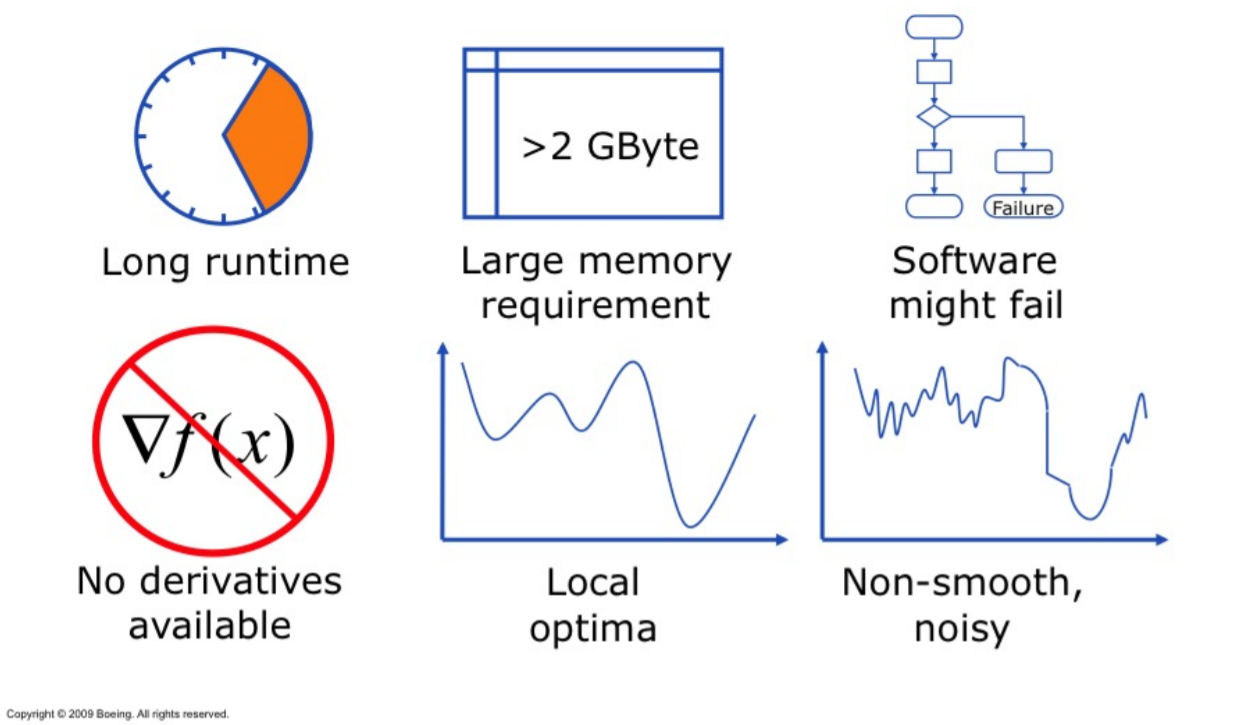
\includegraphics[width=\linewidth]{blackbox.png}
\end{frame}
%%%%%%%%%%%%%%%%%%%%%%%%%%%%%%%%%%%%
%%%%%%% METHODS %%%%%%%%%%
%%%%%%%%%%%%%%%%%%%%%%%%%%%%%%%%%%%%
\begin{frame}
\frametitle{DFO and BBO methods}
\textbf{Trust Region Methods}
\smallskip
% Define block styles
%\tikzstyle{decision} = [diamond, draw, fill=blue!20, 
%text width=4.5em, text badly centered, node distance=3cm, inner sep=0pt]
\tikzstyle{block} = [rectangle, draw, fill=polyblue!20, 
text width=5em, text centered, rounded corners, minimum height=1em]
\tikzstyle{line} = [draw, -latex']
%
\begin{tikzpicture}[node distance = 6.3em, auto]
%% Place nodes
\node [block] (critic) {Criticality Step};
\node [block, right of=critic] (step) {Step Calculation};
\node [block, right of=step] (accept) {Acceptance};
\node [block, right of=accept] (ameliore) {Model Improvement};
\node [block, right of=ameliore] (udate) {T.R. Update};
%% Draw edges
\path [line] (critic) -- (step);
\path [line] (step) -- (accept);
\path [line] (accept) -- (ameliore);
\path [line] (ameliore) -- (udate);
\path [line] (udate) --++ (0cm,-1cm) -| (critic);
\end{tikzpicture}\\
\pause
\smallskip
\textbf{Direct-search Methods}\\
\smallskip
% Define block styles
%\tikzstyle{decision} = [diamond, draw, fill=blue!20, 
%text width=4.5em, text badly centered, node distance=3cm, inner sep=0pt]
\tikzstyle{block} = [rectangle, draw, fill=polyblue!20, 
text width=6em, text centered, rounded corners, minimum height=1em]
\tikzstyle{line} = [draw, -latex']
%
\begin{minipage}[c]{0.45\textwidth}
	\begin{tikzpicture}[node distance = 7.5em, auto]
	%% Place nodes
	\node [block] (sample) {Sampling};
	\node [block, right of=sample] (udate) {Current iterate update};
	%% Draw edges
	\path [line] (sample) -- (udate);
	\path [line] (udate) --++ (0cm,-1cm) -| (sample);
	\end{tikzpicture}
\end{minipage}
\begin{minipage}[c]{0.45\textwidth}
	\begin{itemize}
		\item[]\only<3-7>{Directional (\MADS)}
		\item[]\only<4-7>{Simplicial (Nelder-Mead)}
	\end{itemize}
\end{minipage}\\
\smallskip
\only<5-7>{\textbf{Other methods}}
\begin{itemize}
	\item[]\only<6-7>{Heuristics (Particle Swarm, Simulated Annealing)}
	\item[]\only<7>{Hybrids (Implicit Filtering)}
\end{itemize}
\end{frame} 
%%%%%%%%%%%%%%%%%%%%%%%%%%%%%%%%%%%%
%%%%%%% GOAL              %%%%%%%%%%
%%%%%%%%%%%%%%%%%%%%%%%%%%%%%%%%%%%%
\begin{frame}%6
\frametitle{What Are We Trying to Achieve?}
%Notre but : réduire le nombre d'évaluations d'une boîte noire.
Our goal : reduce the amount of calls to the blackbox
\pause
\medskip

To do so, we consider the \textbf{Opportunistic Strategy}.

\pause
{\begin{block}{Opportunistic Strategy}
%		La stratégie opportuniste désigne l'arrêt prématuré d'une étape d'un l'algorithme si les conditions pour passer à l'étape suivante sont déjà remplies.
The opportunistic strategy designates the premature termination of an algorithmic step as soon as the necessary conditions to proceed to the next step are met.
\end{block}}
\pause
\medskip
Often mentionned but never studied per se.
\end{frame}
%%%%%%%%%%%%%%%%%%%%%%%%%%%%%%%%%%%%
%%%%%%% WHICH METHODS     %%%%%%%%%%
%%%%%%%%%%%%%%%%%%%%%%%%%%%%%%%%%%%%
\section{Direct-search Methods}
\tableofcontents[currentsection,currentsubsection,subsectionstyle=show/hide]
\subsection{Algorithmes}
\begin{frame}
\frametitle{Identifying suitable methods}
\begin{block}{Question 1.}
	For which methods is the opportunistic strategy applicable?
\end{block}
\begin{itemize}
	\item[]\only<2>{Trust Region}\only<3->{{Trust Region} {\color{red}\xmark}}
	\item[]\only<3->{- Only one call to the blackbox per iteration of the method}
	\item[]\only<4>{Simplicial direct-search methods}\only<5->{Simplicial direct-search methods 
		{\color{red}\xmark}}
	\item[]\only<5->{- Already and inevitably opportunistic}
	\item[]\only<6>{Directional direct-search methods}\only<7->{\textbf{Directional direct-search methods} 
		{\checkmarkg}}
	\item[]\only<7->{- Allows opportunistic termination.}
	\item[]\only<8>{Hybrid directional direct-search methods}\only<9->{\textbf{Hybrid directional direct-search methods} \checkmarky}
	\item[]\only<9->{- 
		Same as direct-search methods, but might impact performance.}
	\item[]\only<10>{Heuristics}\only<11->{Heuristics \textbf{\large?}}
	\item[]\only<11->{- Highly dependent on the heuristic.}
\end{itemize}
\end{frame}
%%%%%%%%%%%%%%%%%%%%%%%%%%%%%%%%%%%%
%%%%%%% WHICH METHODS     %%%%%%%%%%
%%%%%%%%%%%%%%%%%%%%%%%%%%%%%%%%%%%%
\begin{frame}%8
\frametitle{Direcitonal direct-search framework}
\textbf{Directional direct-search methods} :
\begin{itemize}
	\pause
	\item Samples $f(x)$ and $c(x)$ on $\L^k$, a list of point specific to the $k^{\text{th}}$ iteration.
	\pause
	\item Generates the next list of candidates $\L^{k+1}$ based on these values.
\end{itemize}
\pause
\setcounter{algorithm}{0}
\begin{minipage}{0.7\linewidth}
	\begin{algorithm}[H]
		\algsetup{linenosize=\tiny}
		\scriptsize
		\begin{algorithmic}[]
			\FOR{$k=1,2,\dots$}
			\STATE \textbf{Search} : Evaluate $f(x)$ at a finite set of point $S^k$.
			\STATE If successful, update $x^k$
			\STATE
			\STATE \textbf{Poll} : Evaluate $f(x)$ at a finite set of point 
			\STATE $P^k:=\{x^k+\delta ^k d:d\in D\}$, where $D$ is a positive spanning set of \textbf{directions}. 
			\STATE If successful, update $x^k$ and mesh parameters.
			\ENDFOR
		\end{algorithmic}
		\caption{Direcitonal direct-search framework}
		\label{alg:seq}
	\end{algorithm}
\end{minipage}\\	
\textit{Remark : this work only encompasses the study of the impact of the opportunistic strategy on poll steps.}
\end{frame}
%%%%%%%%%%%%%%%%%%%%%%%%%%%%%%%%%%%%%%
%%%%%%%%%%%%% EXEMPLE CS %%%%%%%%%%%%%
%%%%%%%%%%%%%%%%%%%%%%%%%%%%%%%%%%%%%%
\begin{frame}
\frametitle{Coordinate Search (\CS)}
\only<1>{
	\begin{minipage}[t]{0.49\linewidth}
		\setcounter{algorithm}{1}
		\begin{algorithm}[H]
			\algsetup{linenosize=\tiny}
			\scriptsize
			\begin{algorithmic}[]
				\FOR{$k=1,2,\dots$}
				\STATE {\textbf{Poll} : Evaluate $f(x)$ at\\
					 $P^k:=\{x^k+\delta ^k d:d\in D_{\oplus}\}$, where\\
					  $D_{\oplus} := \{\pm e_1,\pm e_2,\dots,\pm e_n\}$.}
				\STATE
				\STATE {If $\exists~t$ for which $f(t) < f(x^k)$, $t\in P^k$\\
					 Successful step}
				\STATE update $x^{k+1}\leftarrow t$ et $\delta^{k+1} \leftarrow \delta^k$.
				\STATE
				\STATE {Else $\nexists~t$ for which $f(t) < f(x^k)$, $t\in P^k$\\
				 Unsuccessful step}
				\STATE  update $x^{k+1}\leftarrow x^k$ et $\delta^{k+1} \leftarrow \frac{\delta^k}{2}$.
				\ENDFOR
			\end{algorithmic}
			\caption{Coordinate Search}
			\label{alg:cs}
		\end{algorithm}
	\end{minipage}
	\hfill
	\begin{minipage}[t]{0.49\linewidth}
		\flushleft
		\begin{figure}[H] %FIGURE  : MESH
				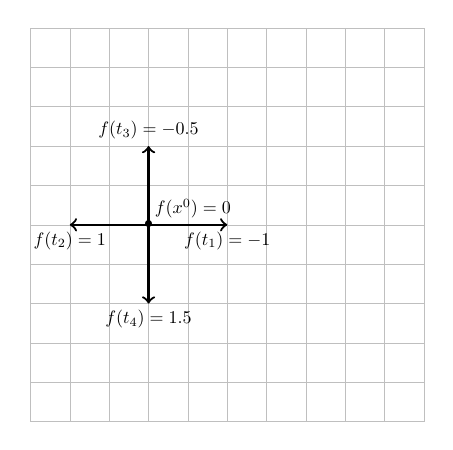
\begin{tikzpicture}
				% Flèches
				\draw [very thin,gray!50] (0,0) grid[step=0.5] (5,5);
				\draw [->,thick] (1.5,2.5)  -- (2.5,2.5) node [below,scale=0.65]{$f(t_1) = -1 $}; 
				\draw [->,thick] (1.5,2.5)  -- (0.5,2.5) node [below,scale=0.65]{$f(t_2) = 1 $}; 
				\draw [->,thick] (1.5,2.5) -- (1.5,3.5) node [above,scale=0.65]{$f(t_3) = -0.5 $};
				\draw [->,thick] (1.5,2.5) -- (1.5,1.5) node [below,scale=0.65]{$f(t_4) = 1.5 $};
				\draw (1.5,2.5) node [above right,scale=0.65]{$f(x^0) = 0$};
				\draw (1.5,2.5) node [scale=0.65] {$\bullet$};
				\end{tikzpicture}
		\caption{\CS}
		\label{fig:CS1}
		\end{figure}
	\end{minipage}}
\only<2>{
	\begin{minipage}[t]{0.49\linewidth}
		\setcounter{algorithm}{1}
				\begin{algorithm}[H]
			\algsetup{linenosize=\tiny}
			\scriptsize
			\begin{algorithmic}[]
				\FOR{$k=1,2,\dots$}
				\STATE {\textbf{Poll} : Evaluate $f(x)$ at\\
					$P^k:=\{x^k+\delta ^k d:d\in D_{\oplus}\}$, where\\
					$D_{\oplus} := \{\pm e_1,\pm e_2,\dots,\pm e_n\}$.}
				\STATE
				\STATE {If $\exists~t$ for which $f(t) < f(x^k)$, $t\in P^k$\\
					Successful step}
				\STATE update $x^{k+1}\leftarrow t$ et $\delta^{k+1} \leftarrow \delta^k$.
				\STATE
				\STATE {Else $\nexists~t$ for which $f(t) < f(x^k)$, $t\in P^k$\\
					Unsuccessful step}
				\STATE  update $x^{k+1}\leftarrow x^k$ et $\delta^{k+1} \leftarrow \frac{\delta^k}{2}$.
				\ENDFOR
			\end{algorithmic}
			\caption{Coordinate Search}
			\label{alg:cs}
		\end{algorithm}
	\end{minipage}
	\hfill
	\begin{minipage}[t]{0.49\linewidth}
		\begin{figure}[H] %FIGURE  : MESH
				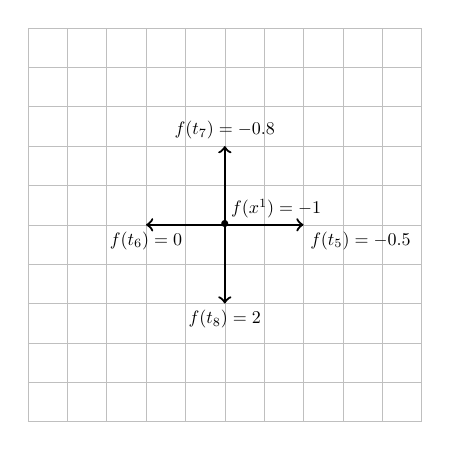
\begin{tikzpicture}
				% Flèches
				\draw [very thin,gray!50] (0,0) grid[step=0.5] (5,5);
				\draw [->,thick] (2.5,2.5)  -- (3.5,2.5) node [below right,scale=0.65]{$f(t_5) = -0.5 $}; 
				\draw [->,thick] (2.5,2.5)  -- (1.5,2.5) node [below,scale=0.65]{$f(t_6) = 0 $}; 
				\draw [->,thick] (2.5,2.5) -- (2.5,3.5) node [above,scale=0.65]{$f(t_7) = -0.8 $};
				\draw [->,thick] (2.5,2.5) -- (2.5,1.5) node [below,scale=0.65]{$f(t_8) = 2 $};
				\draw (2.5,2.5) node [above right,scale=0.65]{$f(x^1) = -1$};
				\draw (2.5,2.5) node [scale=0.65]{$\bullet$};
				\end{tikzpicture}
			\caption{\CS}
			\label{fig:CS2}
		\end{figure}
	\end{minipage}}
\only<3>{
	\begin{minipage}[t]{0.49\linewidth}
		\setcounter{algorithm}{1}
				\begin{algorithm}[H]
			\algsetup{linenosize=\tiny}
			\scriptsize
			\begin{algorithmic}[	]
				\FOR{$k=1,2,\dots$}
				\STATE {\textbf{Poll} : Evaluate $f(x)$ at\\
					$P^k:=\{x^k+\delta ^k d:d\in D_{\oplus}\}$, where\\
					$D_{\oplus} := \{\pm e_1,\pm e_2,\dots,\pm e_n\}$.}
				\STATE
				\STATE {If $\exists~t$ for which $f(t) < f(x^k)$, $t\in P^k$\\
					Successful step}
				\STATE update $x^{k+1}\leftarrow t$ et $\delta^{k+1} \leftarrow \delta^k$.
				\STATE
				\STATE {Else $\nexists~t$ for which $f(t) < f(x^k)$, $t\in P^k$\\
					Unsuccessful step}
				\STATE  update $x^{k+1}\leftarrow x^k$ et $\delta^{k+1} \leftarrow \frac{\delta^k}{2}$.
				\ENDFOR
			\end{algorithmic}
			\caption{Coordinate Search}
			\label{alg:cs}
		\end{algorithm}
	\end{minipage}
	\hfill
	\begin{minipage}[t]{0.49\linewidth}
		\begin{figure}[H] %FIGURE  : MESH
			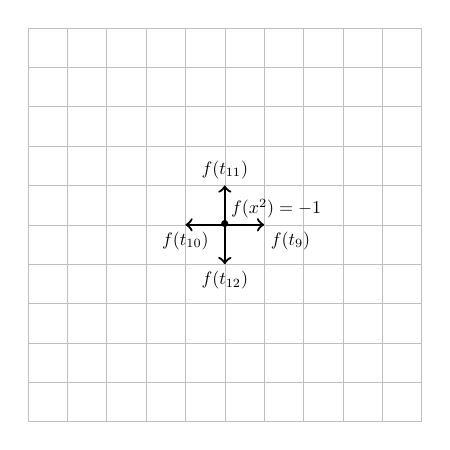
\begin{tikzpicture}
			% Flèches
			\draw [very thin,gray!50] (0,0) grid[step=0.5] (5,5);
			\draw [->,thick] (2.5,2.5)  -- (3,2.5) node [below right,scale=0.65]{$f(t_9)$}; 
			\draw [->,thick] (2.5,2.5)  -- (2,2.5) node [below,scale=0.65]{$f(t_{10})$}; 
			\draw [->,thick] (2.5,2.5) -- (2.5,3) node [above,scale=0.65]{$f(t_{11})$};
			\draw [->,thick] (2.5,2.5) -- (2.5,2) node [below,scale=0.65]{$f(t_{12})$};
			\draw (2.5,2.5) node [above right,scale=0.65]{$f(x^2) = -1$};
			\draw (2.5,2.5) node [scale=0.65]{$\bullet$};
			\end{tikzpicture}
		\caption{\CS}
		\label{fig:CS3}
		\end{figure}
	\end{minipage}}
\end{frame}
%%%%%%%%%%%%%%%%%%%%%%%%%%%%%%%%
%%%%%%%%%%% GPS EXEMPLE %%%%%%%%
%%%%%%%%%%%%%%%%%%%%%%%%%%%%%%%%
\begin{frame}
\frametitle{Generalized Pattern Search (\GPS)}
\only<1>{
	\begin{minipage}[t]{0.49\linewidth}
		\setcounter{algorithm}{2}
		\begin{algorithm}[H]
			\algsetup{linenosize=\tiny}
			\scriptsize
			\begin{algorithmic}[]
				\FOR{$k=1,2,\dots$}
				\STATE with $\tau \in \{0,1\}$.
				\STATE {\textbf{Poll} : Evaluate $f(x)$ at\\
					 $P^k:=\{x^k+\delta ^k d:d\in D\}$, where\\
				{\color{red}$D$ is a positive spanning set.}}
				\STATE
				\STATE {If $\exists~t$ for which $f(t) < f(x^k)$, $t\in P^k$\\
					Successful step}
				\STATE update $x^{k+1}\leftarrow t$ et $\delta^{k+1} \leftarrow {\color{red}\tau^{-1}}\delta^k$.
				\STATE
				\STATE {Else $\nexists~t$ for which $f(t) < f(x^k)$, $t\in P^k$\\
				Unsuccessful step}
				\STATE update $x^{k+1}\leftarrow x^k$ and $\delta^{k+1} \leftarrow {\color{red}\tau}\delta^k$.
				\ENDFOR
			\end{algorithmic}
			\caption{Generalized Pattern Search}
			\label{alg:gps}
		\end{algorithm}
	\end{minipage}
	\hfill
	\begin{minipage}[t]{0.49\linewidth}
		\flushleft
		\begin{figure}[H] %FIGURE  : MESH
			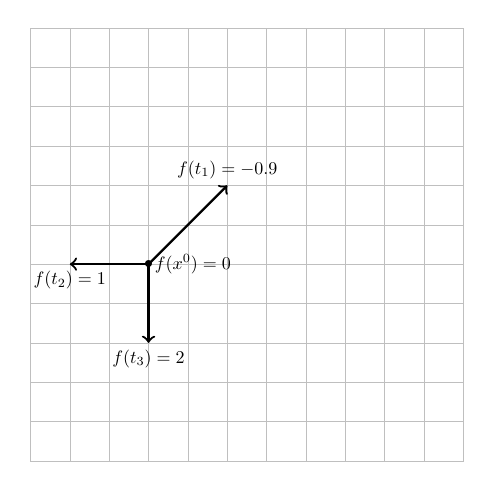
\begin{tikzpicture}
			% Flèches
				\draw [very thin,gray!50] (0,0) grid[step=0.5] (5.5,5.5);
\draw [->,thick] (1.5,2.5) -- (2.5,3.5) node [above,scale=0.65]{$f(t_1) = -0.9 $};
\draw [->,thick] (1.5,2.5)  -- (0.5,2.5) node [below,scale=0.65]{$f(t_2) = 1 $}; 
\draw [->,thick] (1.5,2.5)  -- (1.5,1.5) node [below,scale=0.65]{$f(t_3) = 2 $};
\draw (1.5,2.5) node [right,scale=0.65]{$f(x^0) = 0$};
\draw (1.5,2.5) node [scale=0.65] {$\bullet$};
			\end{tikzpicture}
			\caption{\GPS}
			\label{fig:CS1}
		\end{figure}
\end{minipage}}
\only<2>{
	\begin{minipage}[t]{0.49\linewidth}
		\setcounter{algorithm}{3}
		\begin{algorithm}[H]
			\algsetup{linenosize=\tiny}
			\scriptsize
			\begin{algorithmic}[]
								\FOR{$k=1,2,\dots$}
				\STATE with $\tau \in \{0,1\}$.
				\STATE {\textbf{Poll} : Evaluate $f(x)$ at\\
					$P^k:=\{x^k+\delta ^k d:d\in D\}$, where\\
					{\color{red}$D$ is a positive spanning set.}}
				\STATE
				\STATE {If $\exists~t$ for which $f(t) < f(x^k)$, $t\in P^k$\\
					Successful step}
				\STATE update $x^{k+1}\leftarrow t$ et $\delta^{k+1} \leftarrow {\color{red}\tau^{-1}}\delta^k$.
				\STATE
				\STATE {Else $\nexists~t$ for which $f(t) < f(x^k)$, $t\in P^k$\\
					Unsuccessful step}
				\STATE update $x^{k+1}\leftarrow x^k$ and $\delta^{k+1} \leftarrow {\color{red}\tau}\delta^k$.
				\ENDFOR
			\end{algorithmic}
			\caption{Generalized Pattern Search}
			\label{alg:cs}
		\end{algorithm}
	\end{minipage}
	\hfill
	\begin{minipage}[t]{0.49\linewidth}
		\begin{figure}[H] %FIGURE  : MESH
			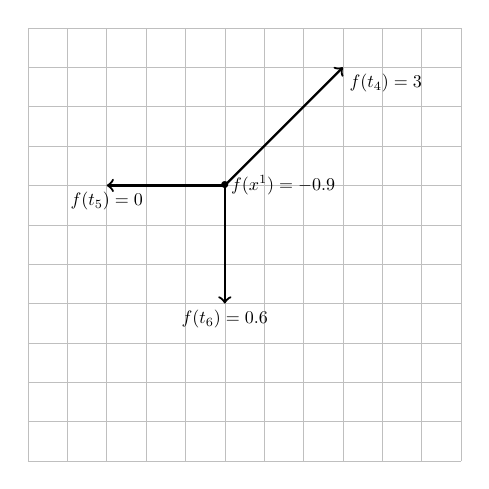
\begin{tikzpicture}
			% Flèches
				\draw [very thin,gray!50] (0,0) grid[step=0.5] (5.5,5.5);
\draw [->,thick] (2.5,3.5) -- (4,5) node [below right,scale=0.65]{$f(t_4) = 3 $};
\draw [->,thick] (2.5,3.5)  -- (1,3.5) node [below,scale=0.65]{$f(t_5) = 0 $}; 
\draw [->,thick] (2.5,3.5)  -- (2.5,2) node [below,scale=0.65]{$f(t_6) = 0.6 $};
\draw (2.5,3.5) node [right,scale=0.65]{$f(x^1) = -0.9$};
\draw (2.5,3.5) node [scale=0.65] {$\bullet$};
			\end{tikzpicture}
			\caption{\GPS}
			\label{fig:CS2}
		\end{figure}
\end{minipage}}
\only<3>{
	\begin{minipage}[t]{0.49\linewidth}
		\setcounter{algorithm}{3}
		\begin{algorithm}[H]
			\algsetup{linenosize=\tiny}
			\scriptsize
			\begin{algorithmic}[	]
				\FOR{$k=1,2,\dots$}
\STATE with $\tau \in \{0,1\}$.
\STATE {\textbf{Poll} : Evaluate $f(x)$ at\\
	$P^k:=\{x^k+\delta ^k d:d\in D\}$, where\\
	{\color{red}$D$ is a positive spanning set.}}
\STATE
\STATE {If $\exists~t$ for which $f(t) < f(x^k)$, $t\in P^k$\\
	Successful step}
\STATE update $x^{k+1}\leftarrow t$ et $\delta^{k+1} \leftarrow {\color{red}\tau^{-1}}\delta^k$.
\STATE
\STATE {Else $\nexists~t$ for which $f(t) < f(x^k)$, $t\in P^k$\\
	Unsuccessful step}
\STATE update $x^{k+1}\leftarrow x^k$ and $\delta^{k+1} \leftarrow {\color{red}\tau}\delta^k$.
\ENDFOR
			\end{algorithmic}
			\caption{Generalized Pattern Search}
			\label{alg:cs}
		\end{algorithm}
	\end{minipage}
	\hfill
	\begin{minipage}[t]{0.49\linewidth}
		\begin{figure}[H] %FIGURE  : MESH
			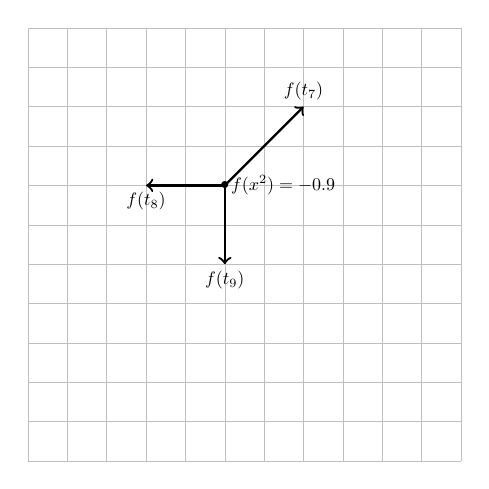
\begin{tikzpicture}
			% Flèches
				\draw [very thin,gray!50] (0,0) grid[step=0.5] (5.5,5.5);
\draw [->,thick] (2.5,3.5) -- (3.5,4.5) node [above,scale=0.65]{$f(t_7)$};
\draw [->,thick] (2.5,3.5)  -- (1.5,3.5) node [below,scale=0.65]{$f(t_8)$}; 
\draw [->,thick] (2.5,3.5)  -- (2.5,2.5) node [below,scale=0.65]{$f(t_9)$};
\draw (2.5,3.5) node [right,scale=0.65]{$f(x^2) = -0.9$};
\draw (2.5,3.5) node [scale=0.65] {$\bullet$};
			\end{tikzpicture}
			\caption{\GPS}
			\label{fig:CS3}
		\end{figure}
\end{minipage}}
\end{frame}
%%%%%%%%%%%%%%%%%%%%%%%%%%%%%55
%%%%%%%%%%%% EXEMPLE GSS %%%%%%
%%%%%%%%%%%%%%%%%%%%%%%%%%%%%%%
\begin{frame}
	\frametitle{Generating Set Search (\GSS)}
	\only<1>{
		\begin{minipage}[t]{0.49\linewidth}
			\setcounter{algorithm}{3}
			\begin{algorithm}[H]
				\algsetup{linenosize=\tiny}
				\scriptsize
				\begin{algorithmic}[]
					\FOR{$k=1,2,\dots$}
					\STATE with $\tau \in \{0,1\}$.
					\STATE {\textbf{Poll} : Evaluate $f(x)$ at\\
						$P^k:=\{x^k+\delta ^k d:d\in D\}$, where\\
						{\color{blue}$D$ is a positive spanning set \\
						respecting multiple conditions.}}
					\STATE
					\STATE {If $\exists~t$ for which $f(t) < f(x^k)$, $t\in P^k$\\
						Successful step}
					\STATE update $x^{k+1}\leftarrow t$ et $\delta^{k+1} \leftarrow {\color{blue}\phi}\delta^k$.
					\STATE
					\STATE {Else $\nexists~t$ for which $f(t) < f(x^k)$, $t\in P^k$\\
						Unsuccessful step}
					\STATE update $x^{k+1}\leftarrow x^k$ and $\delta^{k+1} \leftarrow {\color{red}\tau}\delta^k$.
					\ENDFOR
				\end{algorithmic}
				\caption{Generating Set Search}
				\label{alg:gps}
			\end{algorithm}
		\end{minipage}
		\hfill
		\begin{minipage}[t]{0.49\linewidth}
			\flushleft
			\begin{figure}[H] %FIGURE  : MESH
				\begin{tikzpicture}
				% Flèches
% Flèches
\draw [very thin,white!50] (0,0) grid[step=0.5] (5.5,5.5);
\draw [->,thick] (1.5,2.5) -- (2.5,3.5) node [above,scale=0.65]{$f(t_1) = -0.9 $};
\draw [->,thick] (1.5,2.5)  -- (0.5,2.5) node [below,scale=0.65]{$f(t_2) = 1 $}; 
\draw [->,thick] (1.5,2.5)  -- (1.5,1.5) node [below,scale=0.65]{$f(t_3) = 2 $};
\draw (1.5,2.5) node [right,scale=0.65]{$f(x^0) = 0$};
\draw (1.5,2.5) node [scale=0.65] {$\bullet$};
				\end{tikzpicture}
				\caption{\GSS}
				\label{fig:CS1}
			\end{figure}
	\end{minipage}}
	\only<2>{
		\begin{minipage}[t]{0.49\linewidth}
			\setcounter{algorithm}{3}
						\begin{algorithm}[H]
				\algsetup{linenosize=\tiny}
				\scriptsize
				\begin{algorithmic}[]
					\FOR{$k=1,2,\dots$}
					\STATE with $\tau \in \{0,1\}$.
					\STATE {\textbf{Poll} : Evaluate $f(x)$ at\\
						$P^k:=\{x^k+\delta ^k d:d\in D\}$, where\\
						{\color{blue}$D$ is a positive spanning set \\
							respecting multiple conditions.}}
					\STATE
					\STATE {If $\exists~t$ for which $f(t) < f(x^k)$, $t\in P^k$\\
						Successful step}
					\STATE update $x^{k+1}\leftarrow t$ et $\delta^{k+1} \leftarrow {\color{blue}\phi}\delta^k$.
					\STATE
					\STATE {Else $\nexists~t$ for which $f(t) < f(x^k)$, $t\in P^k$\\
						Unsuccessful step}
					\STATE update $x^{k+1}\leftarrow x^k$ and $\delta^{k+1} \leftarrow {\color{red}\tau}\delta^k$.
					\ENDFOR
				\end{algorithmic}
				\caption{Generating Set Search}
				\label{alg:gps}
			\end{algorithm}
		\end{minipage}
		\hfill
		\begin{minipage}[t]{0.49\linewidth}
			\begin{figure}[H] %FIGURE  : MESH
				\begin{tikzpicture}
				% Flèches
% Flèches
				\draw [very thin,white!50] (0,0) grid[step=0.5] (5.5,5.5);
\draw [->,thick] (2.5,3.5) -- (4,5) node [below right,scale=0.65]{$f(t_4) = 3 $};
\draw [->,thick] (2.5,3.5)  -- (1,3.5) node [below,scale=0.65]{$f(t_5) = 0 $}; 
\draw [->,thick] (2.5,3.5)  -- (2.5,2) node [below,scale=0.65]{$f(t_6) = -0.91 $};
\draw (2.5,3.5) node [right,scale=0.65]{$f(x^1) = -0.9$};
\draw (2.5,3.5) node [scale=0.65] {$\bullet$};
				\end{tikzpicture}
				\caption{\GSS}
				\label{fig:CS2}
			\end{figure}
	\end{minipage}}
	\only<3>{
		\begin{minipage}[t]{0.49\linewidth}
			\setcounter{algorithm}{3}
						\begin{algorithm}[H]
				\algsetup{linenosize=\tiny}
				\scriptsize
				\begin{algorithmic}[]
					\FOR{$k=1,2,\dots$}
					\STATE with $\tau \in \{0,1\}$.
					\STATE {\textbf{Poll} : Evaluate $f(x)$ at\\
						$P^k:=\{x^k+\delta ^k d:d\in D\}$, where\\
						{\color{blue}$D$ is a positive spanning set \\
							respecting multiple conditions.}}
					\STATE
					\STATE {If $\exists~t$ for which $f(t) < f(x^k)$, $t\in P^k$\\
						Successful step}
					\STATE update $x^{k+1}\leftarrow t$ et $\delta^{k+1} \leftarrow {\color{blue}\phi}\delta^k$.
					\STATE
					\STATE {Else $\nexists~t$ for which $f(t) < f(x^k)$, $t\in P^k$\\
						Unsuccessful step}
					\STATE update $x^{k+1}\leftarrow x^k$ and $\delta^{k+1} \leftarrow {\color{red}\tau}\delta^k$.
					\ENDFOR
				\end{algorithmic}
				\caption{Generating Set Search}
				\label{alg:gps}
			\end{algorithm}
		\end{minipage}
		\hfill
		\begin{minipage}[t]{0.49\linewidth}
			\begin{figure}[H] %FIGURE  : MESH
				\begin{tikzpicture}
				% Flèches
% Flèches
				\draw [very thin,white!50] (0,0) grid[step=0.5] (5.5,5.5);
\draw [->,thick] (2.5,3.5) -- (3.25,4.25) node [above,scale=0.65]{$f(t_7)$};
\draw [->,thick] (2.5,3.5)  -- (1.75,3.5) node [below,scale=0.65]{$f(t_8)$}; 
\draw [->,thick] (2.5,3.5)  -- (2.5,2.75) node [below,scale=0.65]{$f(t_9)$};
\draw (2.5,3.5) node [right,scale=0.65]{$f(x^2) = -0.9$};
\draw (2.5,3.5) node [scale=0.65] {$\bullet$};
				\end{tikzpicture}
				\caption{\GSS}
				\label{fig:CS3}
			\end{figure}
	\end{minipage}}
\end{frame}
%%%%%%%%%%%%%%%%%%%%%%%%%%%%%55
%%%%%%%%%%%% EXEMPLE MADS %%%%%%
%%%%%%%%%%%%%%%%%%%%%%%%%%%%%%%
\begin{frame}
\frametitle{Mesh Adaptive Direct Search (\MADS)}
\only<1>{
	\begin{minipage}[t]{0.49\linewidth}
		\setcounter{algorithm}{4}
		\begin{algorithm}[H]
			\algsetup{linenosize=\tiny}
			\scriptsize
			\begin{algorithmic}[]
				\FOR{$k=1,2,\dots$}
				\STATE with $\tau \in \{0,1\}$.
				\STATE {\color{red}Update : $\delta^k \leftarrow \min(\Delta^k,(\Delta^k)^2)$}
				\STATE {\textbf{Poll} : Evaluate $f(x)$ at\\ 
				 $P^k:=\{x^k+\delta ^k d:d\in D\}$, where\\
				  {\color{red}$D\subset F^k$, with 
				  	$F^k$ frame of size $\Delta^k$.}}
				\STATE
				\STATE {If $\exists~t$ for which $f(t) < f(x^k)$, $t\in P^k$\\
				Successful step}
				\STATE update $x^{k+1}\leftarrow t$ et $\delta^{k+1} \leftarrow {\color{blue}\phi}\delta^k$.
				\STATE
				\STATE {Else $\nexists~t$ for which $f(t) < f(x^k)$, $t\in P^k$\\
					Unsuccessful step}
				\STATE update $x^{k+1}\leftarrow x^k$ and $\delta^{k+1} \leftarrow {\color{red}\tau}\delta^k$.
				\ENDFOR
			\end{algorithmic}
			\caption{Mesh Adaptive Direct Search}
			\label{alg:mads}
		\end{algorithm}
	\end{minipage}
	\hfill
	\begin{minipage}[t]{0.49\linewidth}
		\flushleft
		\begin{figure}[H] %FIGURE  : MESH
			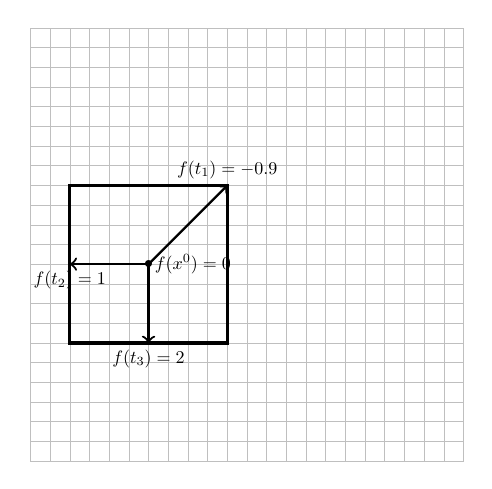
\begin{tikzpicture}
							\draw [very thin,gray!50] (0,0) grid[step=0.25] (5.5,5.5);
			\draw [very thick] (0.5,1.5) rectangle (2.5,3.5);
			\draw [->,thick] (1.5,2.5) -- (2.5,3.5) node [above,scale=0.65]{$f(t_1) = -0.9 $};
			\draw [->,thick] (1.5,2.5)  -- (0.5,2.5) node [below,scale=0.65]{$f(t_2) = 1 $}; 
			\draw [->,thick] (1.5,2.5)  -- (1.5,1.5) node [below,scale=0.65]{$f(t_3) = 2 $};
			\draw (1.5,2.5) node [right,scale=0.65]{$f(x^0) = 0$};
			\draw (1.5,2.5) node [scale=0.65] {$\bullet$};
			\end{tikzpicture}
			\caption{\MADS}
			\label{fig:CS1}
		\end{figure}
\end{minipage}}
\only<2>{
	\begin{minipage}[t]{0.49\linewidth}
\setcounter{algorithm}{4}
\begin{algorithm}[H]
	\algsetup{linenosize=\tiny}
	\scriptsize
	\begin{algorithmic}[]
		\FOR{$k=1,2,\dots$}
		\STATE with $\tau \in \{0,1\}$.
		\STATE {\color{red}Update : $\delta^k \leftarrow \min(\Delta^k,(\Delta^k)^2)$}
		\STATE {\textbf{Poll} : Evaluate $f(x)$ at\\ 
			$P^k:=\{x^k+\delta ^k d:d\in D\}$, where\\
			{\color{red}$D\subset F^k$, with 
				$F^k$ frame of size $\Delta^k$.}}
		\STATE
		\STATE {If $\exists~t$ for which $f(t) < f(x^k)$, $t\in P^k$\\
			Successful step}
		\STATE update $x^{k+1}\leftarrow t$ et $\delta^{k+1} \leftarrow {\color{blue}\phi}\delta^k$.
		\STATE
		\STATE {Else $\nexists~t$ for which $f(t) < f(x^k)$, $t\in P^k$\\
			Unsuccessful step}
		\STATE update $x^{k+1}\leftarrow x^k$ and $\delta^{k+1} \leftarrow {\color{red}\tau}\delta^k$.
		\ENDFOR
	\end{algorithmic}
	\caption{Mesh Adaptive Direct Search}
	\label{alg:mads}
\end{algorithm}
	\end{minipage}
	\hfill
	\begin{minipage}[t]{0.49\linewidth}
		\begin{figure}[H] %FIGURE  : MESH
			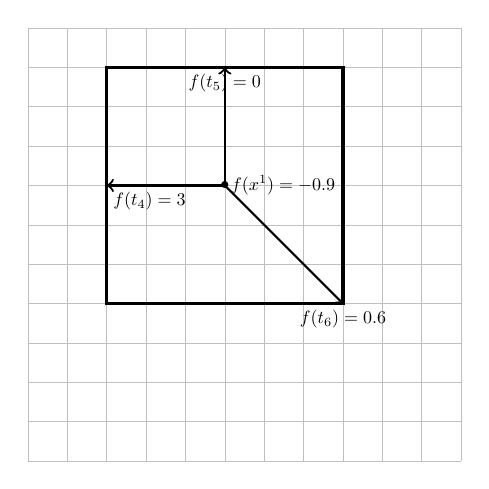
\begin{tikzpicture}
							\draw [very thin,gray!50] (0,0) grid[step=0.5] (5.5,5.5);
			\draw [very thick] (1,2) rectangle (4,5);
			\draw [->,thick] (2.5,3.5) -- (1,3.5) node [below right,scale=0.65]{$f(t_4) = 3 $};
			\draw [->,thick] (2.5,3.5)  -- (2.5,5) node [below,scale=0.65]{$f(t_5) = 0 $}; 
			\draw [->,thick] (2.5,3.5)  -- (4,2) node [below,scale=0.65]{$f(t_6) = 0.6 $};
			\draw (2.5,3.5) node [right,scale=0.65]{$f(x^1) = -0.9$};
			\draw (2.5,3.5) node [scale=0.65] {$\bullet$};
			\end{tikzpicture}
			\caption{\MADS}
			\label{fig:CS2}
		\end{figure}
\end{minipage}}
\only<3>{
	\begin{minipage}[t]{0.49\linewidth}
		\setcounter{algorithm}{4}
		\begin{algorithm}[H]
			\algsetup{linenosize=\tiny}
			\scriptsize
			\begin{algorithmic}[]
				\FOR{$k=1,2,\dots$}
				\STATE with $\tau \in \{0,1\}$.
				\STATE {\color{red}Update : $\delta^k \leftarrow \min(\Delta^k,(\Delta^k)^2)$}
				\STATE {\textbf{Poll} : Evaluate $f(x)$ at\\ 
					$P^k:=\{x^k+\delta ^k d:d\in D\}$, where\\
					{\color{red}$D\subset F^k$, with 
						$F^k$ frame of size $\Delta^k$.}}
				\STATE
				\STATE {If $\exists~t$ for which $f(t) < f(x^k)$, $t\in P^k$\\
					Successful step}
				\STATE update $x^{k+1}\leftarrow t$ et $\delta^{k+1} \leftarrow {\color{blue}\phi}\delta^k$.
				\STATE
				\STATE {Else $\nexists~t$ for which $f(t) < f(x^k)$, $t\in P^k$\\
					Unsuccessful step}
				\STATE update $x^{k+1}\leftarrow x^k$ and $\delta^{k+1} \leftarrow {\color{red}\tau}\delta^k$.
				\ENDFOR
			\end{algorithmic}
			\caption{Mesh Adaptive Direct Search}
			\label{alg:mads}
		\end{algorithm}
	\end{minipage}
	\hfill
	\begin{minipage}[t]{0.49\linewidth}
		\begin{figure}[H] %FIGURE  : MESH
			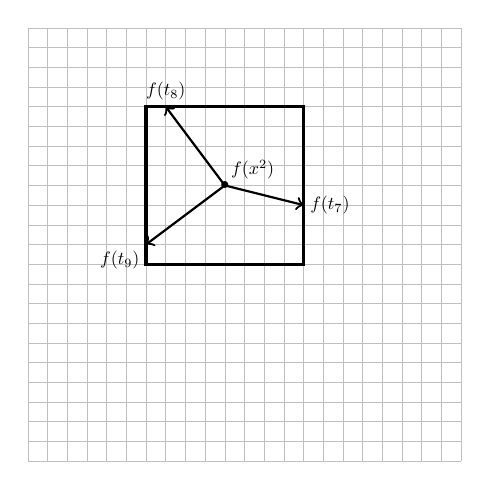
\begin{tikzpicture}
							\draw [very thin,gray!50] (0,0) grid[step=0.25] (5.5,5.5);
			\draw [very thick] (1.5,2.5) rectangle (3.5,4.5);
			\draw [->,thick] (2.5,3.5) -- (3.5,3.25) node [right,scale=0.65]{$f(t_7)$};
			\draw [->,thick] (2.5,3.5)  -- (1.75,4.5) node [above,scale=0.65]{$f(t_8)$}; 
			\draw [->,thick] (2.5,3.5)  -- (1.5,2.75) node [below left,scale=0.65]{$f(t_9)$};
			\draw (2.5,3.5) node [above right,scale=0.65]{$f(x^2)$};
			\draw (2.5,3.5) node [scale=0.65] {$\bullet$};
			\end{tikzpicture}
			\caption{\MADS}
			\label{fig:CS3}
		\end{figure}
\end{minipage}}
\end{frame}
%%%%%%%%%%%%%%%%%%%%%%%%%55
%%%%%%%%%%%%%% imfil
%%%%%%%%%%%%%%%%%%%%%%%%%%%%%
\begin{frame}
\frametitle{Implicit Filtering (\IMFIL)}
\only<1>{
	\begin{minipage}[t]{0.49\linewidth}
		\setcounter{algorithm}{5}
		\begin{algorithm}[H]
			\algsetup{linenosize=\tiny}
			\scriptsize
			\begin{algorithmic}[]
				\FOR{$k=1,2,\dots$}
				\STATE {\textbf{Poll} : Evaluate $f(x)$ at\\
					$P^k:=\{x^k+\delta ^k d:d\in D_{\oplus}\}$, where\\
					$D_{\oplus} := \{\pm e_1,\pm e_2,\dots,\pm e_n\}$.}
				\STATE
				\STATE {If $\exists~t$ for which $f(t) < f(x^k)$, $t\in P^k$\\
					Successful step}
				\STATE {\color{red}Line search following  $-\nabla_s f(x^k)$.}
				\STATE update $x^{k+1}\leftarrow t$ et $\delta^{k+1} \leftarrow \delta^k$.
				\STATE
				\STATE {Else $\nexists~t$ for which $f(t) < f(x^k)$, $t\in P^k$\\
					Unsuccessful step}
				\STATE  update $x^{k+1}\leftarrow x^k$ et $\delta^{k+1} \leftarrow \frac{\delta^k}{2}$.
				\ENDFOR
			\end{algorithmic}
			\caption{Implicit Filtering}
			\label{alg:imfil}
		\end{algorithm}
	\end{minipage}
	\hfill
	\begin{minipage}[t]{0.49\linewidth}
		\flushleft
		\begin{figure}[H] %FIGURE  : MESH
			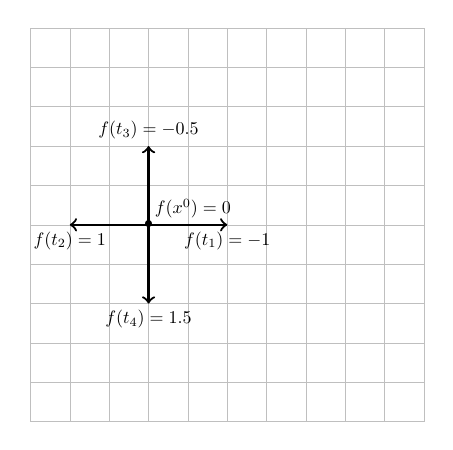
\begin{tikzpicture}
				\draw [very thin,gray!50] (0,0) grid[step=0.5] (5,5);
\draw [->,thick] (1.5,2.5)  -- (2.5,2.5) node [below,scale=0.65]{$f(t_1) = -1 $}; 
\draw [->,thick] (1.5,2.5)  -- (0.5,2.5) node [below,scale=0.65]{$f(t_2) = 1 $}; 
\draw [->,thick] (1.5,2.5) -- (1.5,3.5) node [above,scale=0.65]{$f(t_3) = -0.5 $};
\draw [->,thick] (1.5,2.5) -- (1.5,1.5) node [below,scale=0.65]{$f(t_4) = 1.5 $};
\draw (1.5,2.5) node [above right,scale=0.65]{$f(x^0) = 0$};
\draw (1.5,2.5) node [scale=0.65] {$\bullet$};
			\end{tikzpicture}
			\caption{\IMFIL}
			\label{fig:imfil1}
		\end{figure}
\end{minipage}}
\only<2>{
	\begin{minipage}[t]{0.49\linewidth}
			\setcounter{algorithm}{5}
		\begin{algorithm}[H]
			\algsetup{linenosize=\tiny}
			\scriptsize
			\begin{algorithmic}[]
				\FOR{$k=1,2,\dots$}
				\STATE {\textbf{Poll} : Evaluate $f(x)$ at\\
					$P^k:=\{x^k+\delta ^k d:d\in D_{\oplus}\}$, where\\
					$D_{\oplus} := \{\pm e_1,\pm e_2,\dots,\pm e_n\}$.}
				\STATE
				\STATE {If $\exists~t$ for which $f(t) < f(x^k)$, $t\in P^k$\\
					Successful step}
				\STATE {\color{red}Line search following  $-\nabla_s f(x^k)$.}
				\STATE update $x^{k+1}\leftarrow t$ et $\delta^{k+1} \leftarrow \delta^k$.
				\STATE
				\STATE {Else $\nexists~t$ for which $f(t) < f(x^k)$, $t\in P^k$\\
					Unsuccessful step}
				\STATE  update $x^{k+1}\leftarrow x^k$ et $\delta^{k+1} \leftarrow \frac{\delta^k}{2}$.
				\ENDFOR
			\end{algorithmic}
			\caption{Implicit Filtering}
			\label{alg:imfil}
		\end{algorithm}
	\end{minipage}
	\hfill
	\begin{minipage}[t]{0.49\linewidth}
		\begin{figure}[H] %FIGURE  : MESH
			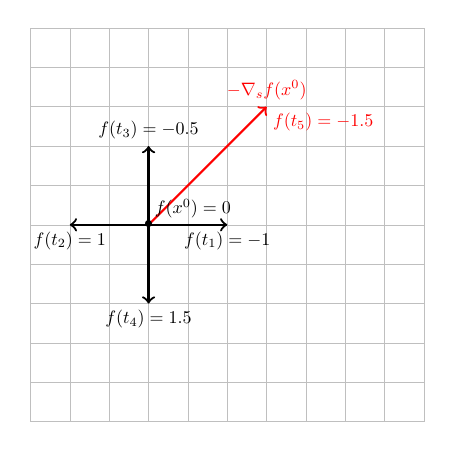
\begin{tikzpicture}
				\draw [very thin,gray!50] (0,0) grid[step=0.5] (5,5);
\draw [->,thick] (1.5,2.5)  -- (2.5,2.5) node [below,scale=0.65]{$f(t_1) = -1 $}; 
\draw [->,thick] (1.5,2.5)  -- (0.5,2.5) node [below,scale=0.65]{$f(t_2) = 1 $}; 
\draw [->,thick] (1.5,2.5) -- (1.5,3.5) node [above,scale=0.65]{$f(t_3) = -0.5 $};
\draw [->,thick] (1.5,2.5) -- (1.5,1.5) node [below,scale=0.65]{$f(t_4) = 1.5 $};
\draw [->,thick,red] (1.5,2.5) -- (3,4) node [above, scale = 0.65]{$-\nabla_sf(x^0)$};
\draw [red] (3,4) node [below right,scale=0.65]{$f(t_5) = -1.5$};
\draw (1.5,2.5) node [above right,scale=0.65]{$f(x^0) = 0$};
\draw (1.5,2.5) node [scale=0.65] {$\bullet$};
			\end{tikzpicture}
			\caption{\IMFIL}
			\label{fig:CS2}
		\end{figure}
\end{minipage}}
\only<3>{
	\begin{minipage}[t]{0.49\linewidth}
		\setcounter{algorithm}{5}
	\begin{algorithm}[H]
		\algsetup{linenosize=\tiny}
		\scriptsize
		\begin{algorithmic}[]
			\FOR{$k=1,2,\dots$}
			\STATE {\textbf{Poll} : Evaluate $f(x)$ at\\
				$P^k:=\{x^k+\delta ^k d:d\in D_{\oplus}\}$, where\\
				$D_{\oplus} := \{\pm e_1,\pm e_2,\dots,\pm e_n\}$.}
			\STATE
			\STATE {If $\exists~t$ for which $f(t) < f(x^k)$, $t\in P^k$\\
				Successful step}
			\STATE {\color{red}Line search following  $-\nabla_s f(x^k)$.}
			\STATE update $x^{k+1}\leftarrow t$ et $\delta^{k+1} \leftarrow \delta^k$.
			\STATE
			\STATE {Else $\nexists~t$ for which $f(t) < f(x^k)$, $t\in P^k$\\
				Unsuccessful step}
			\STATE  update $x^{k+1}\leftarrow x^k$ et $\delta^{k+1} \leftarrow \frac{\delta^k}{2}$.
			\ENDFOR
		\end{algorithmic}
		\caption{Implicit Filtering}
		\label{alg:imfil}
	\end{algorithm}
	\end{minipage}
	\hfill
	\begin{minipage}[t]{0.49\linewidth}
		\begin{figure}[H] %FIGURE  : MESH
			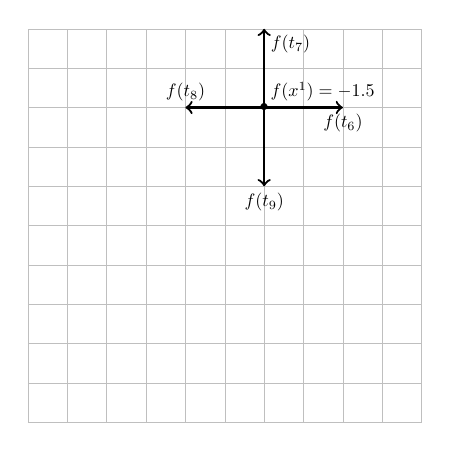
\begin{tikzpicture}
				\draw [very thin,gray!50] (0,0) grid[step=0.5] (5,5);
\draw [->,thick] (3,4)  -- (4,4) node [below,scale=0.65]{$f(t_6)$}; 
\draw [->,thick] (3,4)  -- (3,5) node [below right,scale=0.65]{$f(t_7)$}; 
\draw [->,thick] (3,4) -- (2,4) node [above,scale=0.65]{$f(t_8)$};
\draw [->,thick] (3,4) -- (3,3) node [below,scale=0.65]{$f(t_9)$};
\draw (3,4) node [above right,scale=0.65]{$f(x^1) = -1.5$};
\draw (3,4) node [scale=0.65] {$\bullet$};
			\end{tikzpicture}
			\caption{\IMFIL}
			\label{fig:CS3}
		\end{figure}
\end{minipage}}
\end{frame}
%%%%%%%%%%%%%%%%%%%%%%%%%%%%%%%%%%%%
\section{Opportunism and ordering}
\tableofcontents[currentsection,currentsubsection,subsectionstyle=show/hide]
\subsection{Opportunism}
\begin{frame}
\frametitle{Opportunistic strategies}
{\begin{block}{Complete polling}\small
		Designates the evaluation of $f(x)$ and $c(x)$ at every point generated in the poll step.
\end{block}}
\pause
\medskip
\begin{block}{Simple opportunistic strategy}\small
	Designates the opportunistic termination of the poll after \textbf{a single successful point} 
\end{block}
\pause
\medskip
\begin{block}{Opportunistic strategy after $p$ success}\small
	Opportunistic termination of the poll following the evaluation of \textbf{$p$} successful points.
\end{block}
\pause
\medskip
{\begin{block}{Opportunistic strategy after $q$ evaluations}\small
	Opportunistic termination of the poll following the evaluations of \textbf{$q$} points.\end{block}}
\end{frame}
%%%%%%%%%%%%%%%%%%%%%%%%%%%%%%%
%%%%%%%% DEFINITIONS
%%%%%%%%%%%%%%%%%%%%%%%%%%%%%%%
\begin{frame}
\frametitle{Ordering strategies}
\begin{block}{Ordering strategy}
		Rule guiding the ordering of points in a set $\L$.
\end{block}
\begin{enumerate}
\item\only<1->{\textbf{Lexicographic}}
\pause
\item[]\only<2->{Ordered as in a dictionary, i.e. $(0,0,1)\prec (0,0,3) \prec (0,1,0)$.}
\pause
\item\only<3->{\textbf{Random}}
\pause
\item\only<4->{\textbf{Last success direction}}
\pause
\item[]\only<5->{Ordered by the angle made with the last successful point's corresponding direction}
\pause
\item\only<6->{\textbf{Quadratic models}}
\pause
\item[]\only<7->{$A\prec B$ if $\tilde{f}(A) < \tilde{f}(B)$}
\item[]\only<8->{where $\tilde{f}(x)$ is a dynamic quadratic surrogate of $f(x)$.}
\end{enumerate}
\end{frame}
%%%%%%%%%%%%%%%%%%%%%%%%%%%%%%%
%%%%%%%% OMNISCIENT STRATEGIES
%%%%%%%%%%%%%%%%%%%%%%%%%%%%%%%%
\begin{frame}
\frametitle{Omniscient strategies}
Use $f(x)$ as a surrogate for $f(x)$ to simulate the best ordering possible.
\pause
\begin{itemize}
	\item[\mynum{5}]\only<2->{\textbf{Omniscient}}
	\pause
	\item[]\only<3->{$A \prec B$ if $f(A)<f(B)$}
\end{itemize}
\pause
\bigskip
\only<4->{Use $-f(x)$ as a surrogate for $f(x)$ to simulate the worst ordering possible.}
\pause
\begin{enumerate}
	\item[\mynum{6}]\only<5->{\textbf{Reverse Omniscient}}
	\pause
	\item[]\only<6->{$A \prec B$ if $f(A)>f(B)$}
\end{enumerate}
\bigskip
\pause

\begin{center}
	{\color{red} \Large No practical use, for comparaison only.}
\end{center}
\end{frame}
%%%%%%%%%%%%%%%%%%%%%%%%%%%%%%%
%%%%%%%% NUMERICAL RESULTS
%%%%%%%%%%%%%%%%%%%%%%%%%%%%%%%%
\section{Numerical results}
\tableofcontents[currentsection,currentsubsection,subsectionstyle=show/hide]
\subsection{Numerical results}
\begin{frame}
\frametitle{Test problems}
\begin{enumerate}
	\item\only<1->{212 instances of problems taken from \cite{MoWi2009}}
	\pause
	\item\only<2->{18 constrained problems taken from \cite{AuTr17}}
	\pause 
	\item[]\only<3->{Infeasable starting point $x^0$}
	\pause
	\item\only<4->{A blackbox taken from \cite{AuBeLe08}}
	\pause
	\item[]\only<5->{$f:R^8\mapsto R$, $c:R^8\mapsto R^{11}$, 4 binary constraints, 7 relaxables constraints}
\end{enumerate}
\pause
\begin{center}
	\begin{figure}
		\centering
		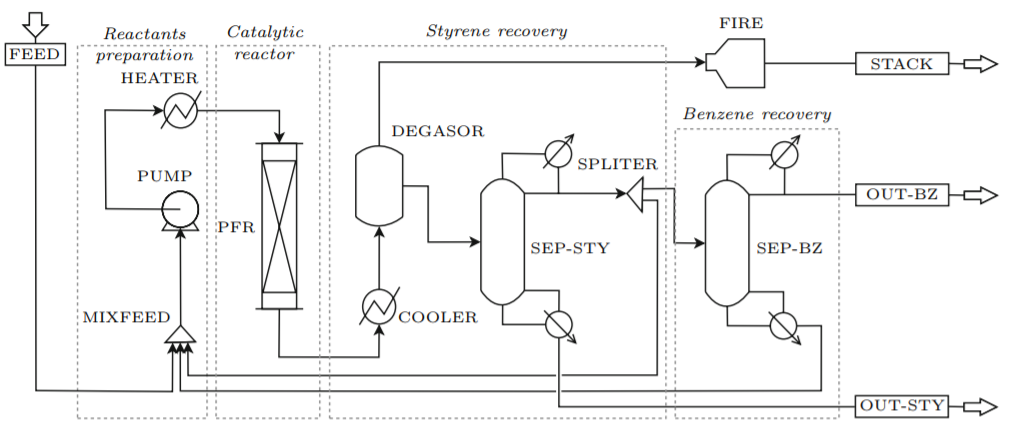
\includegraphics[width=7cm]{StyreneFlow.PNG}
		\caption{Styrene production chart \cite{AuBeLe08}}
	\end{figure}
\end{center}
\end{frame}
\begin{frame}
%%%%%%%%%%%%%%%%%%%%%%%%%%%%%%
%%%%%%%%%% Comparison of opp. strategies
%%%%%%%%%%%%%%%%%%%%%%%%%%%%%%%
\frametitle{Opportunistic strategies comparison}
\noindent
\begin{center}
	\begin{figure}
		\vspace{-1em}
		\begin{minipage}[t]{0.45\linewidth}
			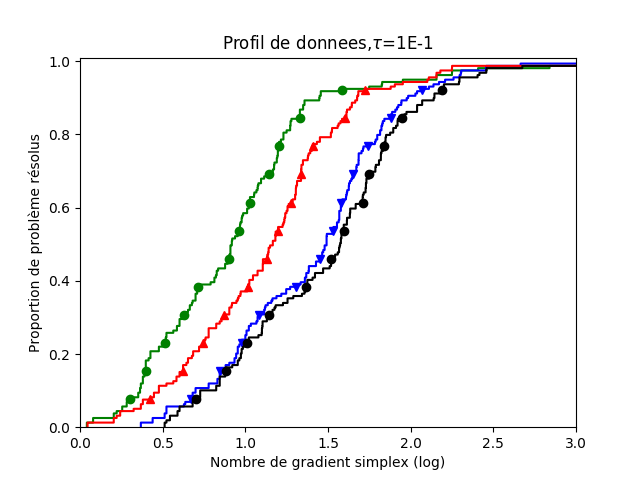
\includegraphics[width=\linewidth]{coppcomp.png}
		\end{minipage}
		\hfill%
		\begin{minipage}[t]{0.45\linewidth}
			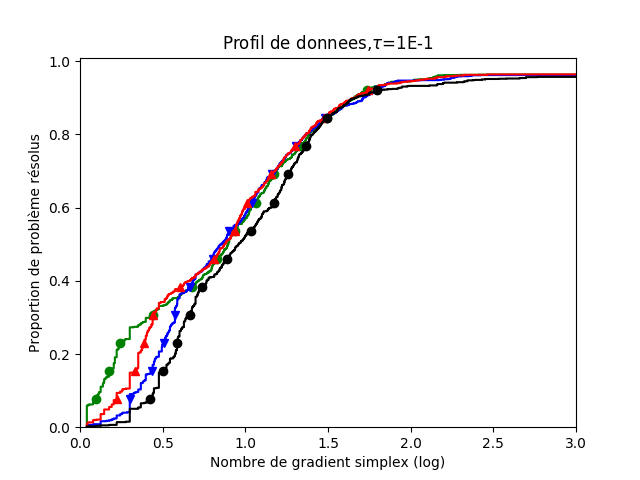
\includegraphics[width=\linewidth]{moppcomp.png}
		\end{minipage}
		
\includegraphics[width=\linewidth]{Legende_comp.png}
		\vspace{-1.5em}
		\caption{Left : \CS~on Moré-Wild, Right \MADS~on Moré-Wild}
		\vspace{-1.3em}
	\end{figure}
\end{center}
\begin{minipage}[t]{0.5\linewidth}
	\begin{enumerate}
		\pause
		\item Model ordering used.
		\pause
		\item Most efficient opprtunistic strategy : simple
	\end{enumerate}
\end{minipage}%
\hfill%
\begin{minipage}[t]{0.5\linewidth}
	\begin{enumerate}
		\pause
		\item[\mynum{3}] Impact less important on \MADS.
	\end{enumerate}
\end{minipage}
\end{frame}
%%%%%%%%%%%%%%%%%%%%%%%%%%%%%%%%%%%%%%%%%%%%%%%%%%55
%%%%%%%%%%%%%%%%%%%%%%%%%% comparaison on cs
%%%%%%%%%%%%%%%%%%%%%%%%%55
\begin{frame}
\frametitle{Ordering strategies comparison}
\noindent
	\begin{center}
		\begin{figure}
			\vspace{-1em}
			\begin{minipage}[t]{0.5\linewidth}
				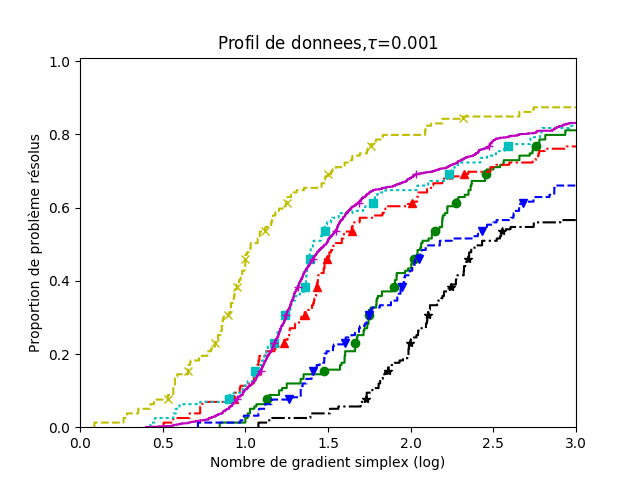
\includegraphics[width=\linewidth]{cog.png}
			\end{minipage}\\
			
\includegraphics[width=\linewidth]{legende_mw.png}
			\vspace{-1em}
			\caption{\CS~on Moré-Wild}
			\vspace{-1.3em}
		\end{figure}
	\end{center}
\end{frame}
%%%%%%%%%%%%%%%%%%%%%%%%%%%%%%%%%%%%%%%%%%%%%%%
%%%%%%%%%%% comparison on GPS
%%%%%%%%%%%%%%%%%%%%%%%%%%%%%%%%%%%%%%%%%%%%%%
\begin{frame}
\frametitle{Ordering strategies comparison}
\noindent
\begin{center}
	\begin{figure}
		\vspace{-1em}
		\begin{minipage}[t]{0.5\linewidth}
			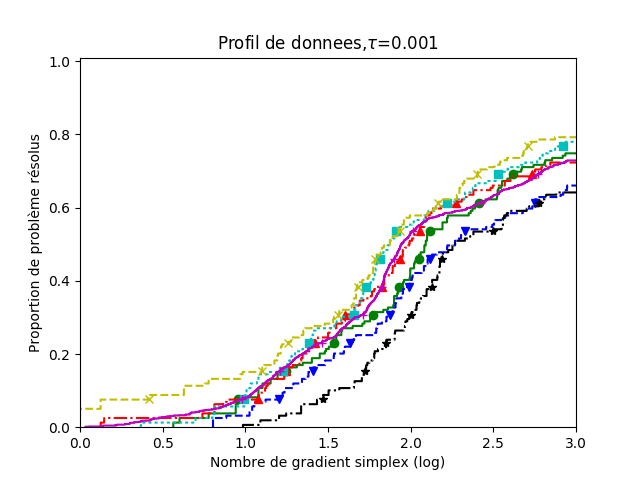
\includegraphics[width=\linewidth]{gog.png}
		\end{minipage}\\
		%
		%\begin{minipage}[t]{0.5\linewidth}
		%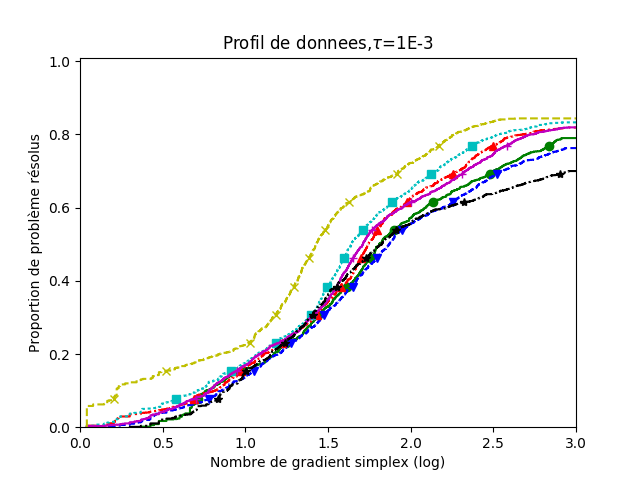
\includegraphics[width=\linewidth]{mog.png}
		%\end{minipage}
		
\includegraphics[width=\linewidth]{legende_mw.png}
		\vspace{-1em}
		\caption{\GPS~on Moré-Wild}
		\vspace{-1.3em}
	\end{figure}
\end{center}
\begin{minipage}[t]{0.5\linewidth}
	\begin{enumerate}
		\pause
		\item Omniscient strategy less dominant.
	\end{enumerate}
\end{minipage}%
\hfill%
\begin{minipage}[t]{0.5\linewidth}
	\begin{enumerate}
		\pause
		\item[\mynum{2}] Somewhat similar hierarchy.
		%\pause
		%\item[\mynum{3}] Impact moins important sur \MADS.
		%\pause
		%\item[\mynum{4}] Classement différent sur \CS~ et \MADS.
	\end{enumerate}
\end{minipage}
\end{frame}
%%%%%%%%%%%%%%%%%%%%%%%%%%%%%%%%%%%%%%%%%%%%%%%%%%%%%%%%%
%%%%%%%%%%%%%%%% MADS comparison
%%%%%%%%%%%%%%%%%%%%%%%%%%%%%%%%%%%%%%%%%%%%%%%%%%%%%%%%%
\begin{frame}
\frametitle{Ordering strategies comparison}
\noindent
\begin{center}
	\begin{figure}
		\vspace{-1em}
		\begin{minipage}[t]{0.5\linewidth}
			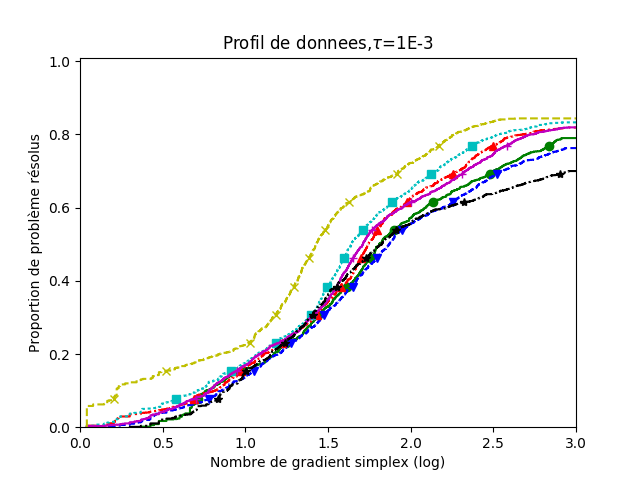
\includegraphics[width=\linewidth]{mog.png}
		\end{minipage}\\
		%
		%\begin{minipage}[t]{0.5\linewidth}
		%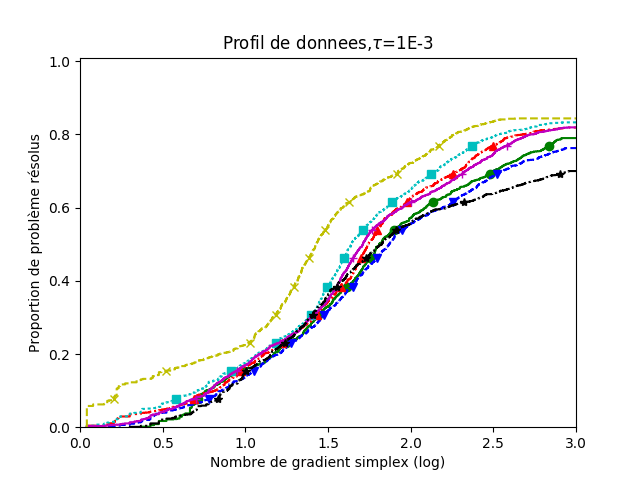
\includegraphics[width=\linewidth]{mog.png}
		%\end{minipage}
		
\includegraphics[width=\linewidth]{legende_mw.png}
		\vspace{-1em}
		\caption{\MADS~on Moré-Wild}
		\vspace{-1.3em}
	\end{figure}
\end{center}
\begin{minipage}[t]{0.5\linewidth}
	\begin{enumerate}
		\pause
		\item Impact less visible on \MADS.
	\end{enumerate}
\end{minipage}%
\hfill%
\begin{minipage}[t]{0.5\linewidth}
	\begin{enumerate}
		\pause
		\item[\mynum{2}] Different ranking of strategies on \CS~ and \MADS.
		%\pause
		%\item[\mynum{3}] Impact moins important sur \MADS.
		%\pause
		%\item[\mynum{4}] Classement différent sur \CS~ et \MADS.
	\end{enumerate}
\end{minipage}
\end{frame}
%%%%%%%%%%%%%%%%%%%%%%%%%%%%%%%%%%%%%%%%%%%%%%%%%%%%%%%%
%%%%%%%%%%%%%%%%%%%%%%%% IMFIL %%%%%%%%%%%%%%%%%%%%%%%%%
%%%%%%%%%%%%%%%%%%%%%%%%%%%%%%%%%%%%%%%%%%%%%%%%%%%%%%%%
\begin{frame}
\frametitle{Ordering strategies comparison}
\noindent
\begin{center}
	\begin{figure}
		\vspace{-1em}
		\begin{minipage}[t]{0.5\linewidth}
			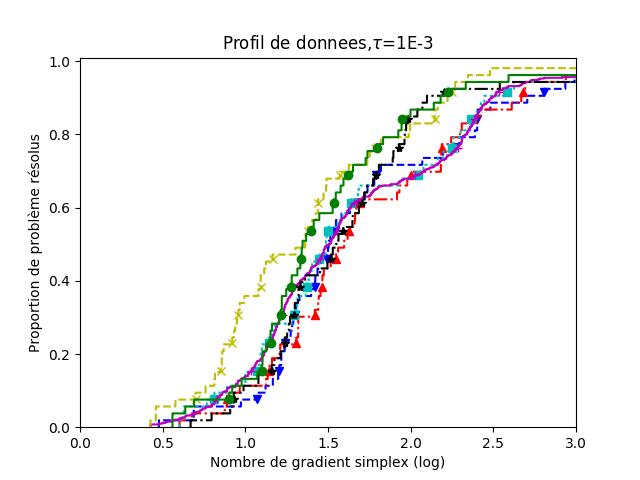
\includegraphics[width=\linewidth]{imfil.png}
		\end{minipage}\\
		
\includegraphics[width=\linewidth]{legende_mw.png}
		\vspace{-1.5em}
		\caption{\IMFIL~on Moré-Wild}
		\vspace{-1.3em}
	\end{figure}
\end{center}
\begin{minipage}[t]{0.5\linewidth}
	\begin{enumerate}
		\pause
		\item Opportunism profitable with omniscient and reverse-omniscient only.
	\end{enumerate}
\end{minipage}%
\hfill%
\begin{minipage}[t]{0.5\linewidth}
	\begin{enumerate}
		\pause
		\item[\mynum{2}] Opportunism is harmful with the available realistic strategies.
	\end{enumerate}
\end{minipage}
\end{frame}
%%%%%%%%%%%%%%%%%%%%%%%%%%%%%%%%%%%%%%%%%%%
%%%%%%%% Constrained problems with mads
%%%%%%%%%%%%%%%%%%%%%%%%%%%%%%%%%%%%%%%%%
\begin{frame}
\frametitle{Ordering strategies comparison}
\noindent
\begin{center}
	\begin{figure}
		\vspace{-1em}
		\begin{minipage}[t]{0.5\linewidth}
			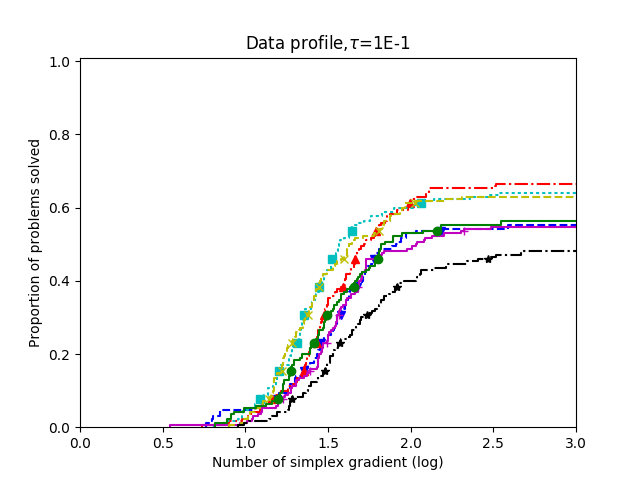
\includegraphics[width=\linewidth]{const.png}
		\end{minipage}
		
\includegraphics[width=\linewidth]{legende_mw.png}
		\vspace{-1.5em}
		\caption{Constrained problems with \MADS}
		\vspace{-1.3em}
	\end{figure}
\end{center}

\begin{center}
	\begin{enumerate}
		\pause
		\item[\mynum{1}] Omniscient strategy not as good as using the direction of the last success.
		\pause
		\item[\mynum{2}] Surrogate ordering with progressive barrier might not be optimal.
	\end{enumerate}
\end{center}
\end{frame}
%%%%%%%%%%%%%%%%%%%%%%%%%%%%%%
%%%%%%%%% Styrene 1 %%%%%%%%%%
%%%%%%%%%%%%%%%%%%%%%%%%%%%%%%
\begin{frame}
\noindent
\frametitle{Ordering strategies comparison}
\begin{center}
	\begin{figure}
		\vspace{-1em}
		\begin{minipage}[t]{0.5\linewidth}
			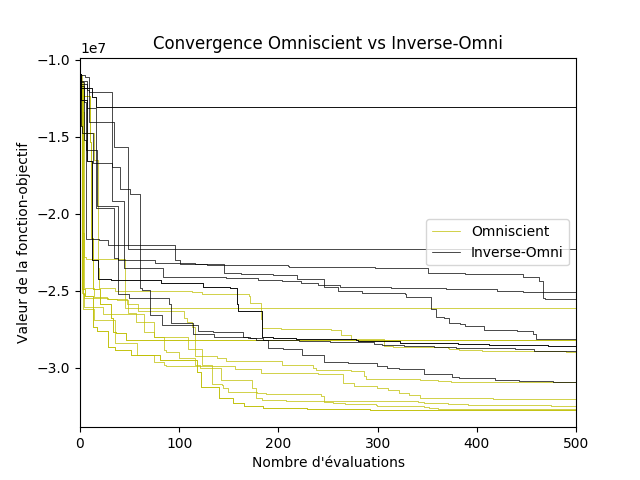
\includegraphics[width=\linewidth]{sty1.png}
		\end{minipage}%
		\hfill%
		\begin{minipage}[t]{0.5\linewidth}
			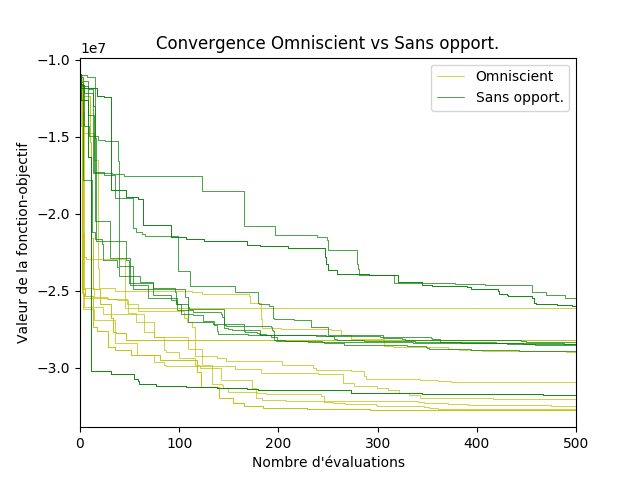
\includegraphics[width=\linewidth]{sty2.png}
		\end{minipage}
		\vspace{-1.5em}
		\caption{Comparing omniscient, reverse-omniscient and complete polling}
		\vspace{-1em}
	\end{figure}
	\begin{enumerate}
		\pause
		\item Omniscient strategy converges to a different solution.
		\pause
		\item[\mynum{2}] Complete polling ressembles reverse-omniscient.
	\end{enumerate}
\end{center}
\end{frame}
%%%%%%%%%%%%%%%%%%%%%%%%%%%%%%%%%%%%%
%%%%%%%%%%%%%%%% Styrene v2%%%%%%%%%%%
%%%%%%%%%%%%%%%%%%%%%%%%%%%%%%%%%%%%%
\begin{frame}
\frametitle{Ordering strategies comparison}
\noindent
\begin{center}
	\begin{figure}
		\vspace{-1em}
		\begin{minipage}[t]{0.5\linewidth}
			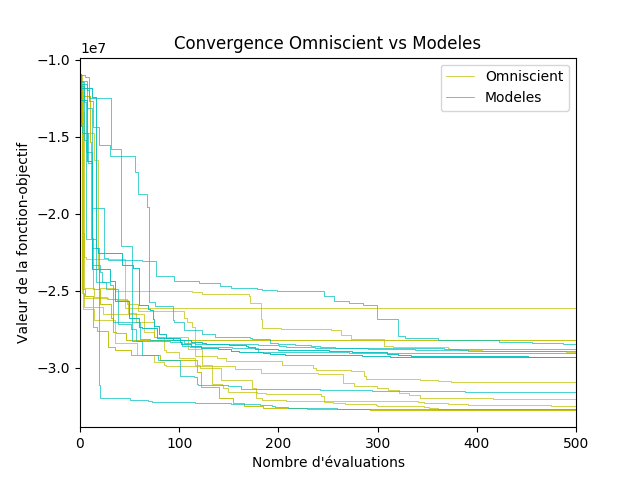
\includegraphics[width=\linewidth]{sty3.png}
		\end{minipage}%
		\hfill%
		\begin{minipage}[t]{0.5\linewidth}
			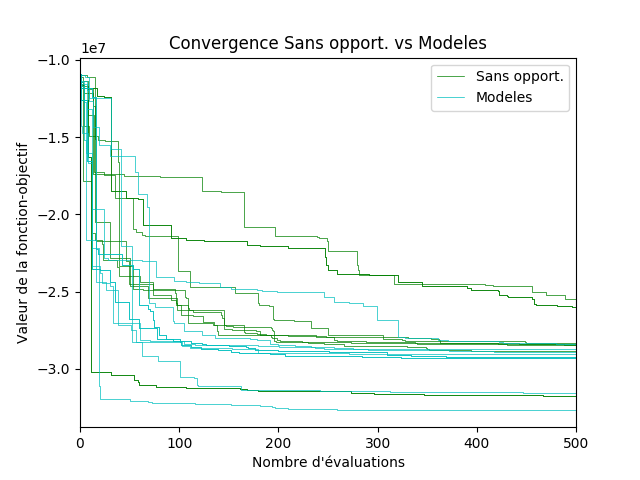
\includegraphics[width=\linewidth]{sty4.png}
		\end{minipage}
		\vspace{-1.5em}
		\caption{Comparing omniscient, model ordering and complete polling}
		\vspace{-1em}
	\end{figure}
	\begin{enumerate}
		\pause
		\item Model ordering converges faster than complete polling.
		\pause
		\item Model ordering converges to a solution different from the one obtained from the omniscient ordering.
	\end{enumerate}
\end{center}
\end{frame}
\section{Conclusion}
\tableofcontents[currentsection,currentsubsection,subsectionstyle=show/hide]
\subsection{Conclusion}
%%%%%%%%%%%%%%%%%%%%%%%%%%%%%%%%%
%%%%%%%%%%% resume %%%%%%%%%%%%%%
%%%%%%%%%%%%%%%%%%%%%%%%%%%%%%%%%\section{Conclusion}
\tableofcontents[currentsection,currentsubsection,subsectionstyle=show/hide]
\subsection{Conclusion}
\begin{frame}
\frametitle{Summary}
\begin{itemize}
	\item\only<1->{In general, the opportunistic strategy benefits to directionnal direct-search methods.}
	\pause
	\item\only<1>{~}\only<2->{Opportunism can deteriorate a method's performance if coupled with an inadequate ordering strategy.}
	\pause
	\item\only<1-2>{~}\only<3->{The more the poll step is refined the less opportunistism impacts it.}
	\pause
	\item\only<1-3>{~}\only<4->{Strategies other than simple opportunism tend to behave like complete polling.}
	\pause
	\item\only<1-4>{~}\only<5->{Ranking of strategies on unconstrained problems : Models, Random/Last success direction, Complete polling and Lexicographic ordering.}
	\pause
	\item\only<1-5>{~}\only<6->{For \IMFIL, the opportunistic strategy is harmful.}
\end{itemize}
\end{frame}

\begin{frame}
\frametitle{Future work}
There is room for improvement in ordering strategies.
\pause
\begin{itemize}
\item\only<2->{Use other kind of models.}
\pause
\item\only<2>{~}\only<3->{Identify more ordering strategies (Distance from the solution of a model.)}
\pause
\item\only<2-3>{~}\only<4->{Identify more strategies in relation with the progressive barrier.}
\pause
\item\only<2-4>{~}\only<5->{Use minimal decrease as an opportunism criteria.}
\pause
\item\only<2-5>{~}\only<6->{Opportunism and parallelism.}
\end{itemize}
\end{frame}
\begin{frame}
\frametitle{Summary}
\begin{itemize}
	\item\only<1->{In general, the opportunistic strategy benefits to directionnal direct-search methods.}
	\pause
	\item\only<1>{~}\only<2->{Opportunism can deteriorate a method's performance if coupled with an inadequate ordering strategy.}
	\pause
	\item\only<1-2>{~}\only<3->{The more the poll step is refined the less opportunistism impacts it.}
	\pause
	\item\only<1-3>{~}\only<4->{Strategies other than simple opportunism tend to behave like complete polling.}
	\pause
	\item\only<1-4>{~}\only<5->{Ranking of strategies on unconstrained problems : Models, Random/Last success direction, Complete polling and Lexicographic ordering.}
	\pause
	\item\only<1-5>{~}\only<6->{For \IMFIL, the opportunistic strategy is harmful.}
\end{itemize}
\end{frame}
%%%%%%%%%%%%%%%%%%%%%%%%%%%%%
%%%%%%%%%%% FUTURE WORK%%%%%%%%%%
\begin{frame}
\frametitle{Future work}
There is room for improvement in ordering strategies.
\pause
\begin{itemize}
\item\only<2->{Use other kind of models.}
\pause
\item\only<2>{~}\only<3->{Identify more ordering strategies (Distance from the solution of a model.)}
\pause
\item\only<2-3>{~}\only<4->{Identify more strategies in relation with the progressive barrier.}
\pause
\item\only<2-4>{~}\only<5->{Use minimal decrease as an opportunism criteria.}
\pause
\item\only<2-5>{~}\only<6->{Opportunism and parallelism.}
\end{itemize}
\end{frame}
\begin{frame}
%%%%%%%%%%%%% bibligraPHY
\frametitle{References}
\footnotesize{
	\begin{thebibliography}{99} % Beamer does not support BibTeX so references must be nserted manually as below
		\bibitem[J.J. Mor\'e and S.M. Wild 2009]{MoWi2009} J.J. Mor\'e and S.M. Wild (2009)
		\newblock   Benchmarking Derivative-Free Optimization Algorithms
		\newblock \emph{SIAM Journal on Optimization} 20(1). 172--191
		
		\bibitem[Audet, Tribes, 2017]{AuTr17} C. Audet and C. Tribes (2017)
		\newblock Mesh-based Nelder-Mead algorithm for inequality constrained
		optimization
		\newblock \emph{Les Cahiers du Gerad} G-2017-90.
		
		\bibitem[Audet, Béchard, Le Digabel 2008]{AuBeLe08}C. Audet and V. B\'echard and S. {Le~Digabel} (2008)
		\newblock Nonsmooth optimization through Mesh Adaptive Direct Search
		and Variable Neighborhood Search
		\newblock \emph{Journal of Global Optimization} 41-2.
		
		\bibitem[Le Digabel 2009]{Le09b} S. {Le~Digabel} (2009)
		\newblock Algorithm 909: NOMAD: Nonlinear Optimization with the MADS algorithm
		\newblock \emph{{ACM} Transactions on Mathematical Software} 37-4.
	\end{thebibliography}
}
\end{frame}
\begin{frame}
	\frametitle{~}
	\centering
	{\LARGE \textbf{QUESTIONS?}}
\end{frame}
\end{document}